\documentclass[11pt]{report}

\usepackage{polski}
\usepackage[utf8]{inputenc}
\usepackage{geometry}
\newgeometry{left=0.8in,right=0.8in,top=1in,bottom=1in}
\usepackage{graphicx}
\usepackage{subcaption}
\usepackage{float}
\usepackage{amssymb}
\usepackage{flexisym}
\renewcommand{\thesection}{\arabic{section}.}
\renewcommand{\thesubsection}{\arabic{section}.\arabic{subsection}.}
\usepackage{makecell}
\usepackage[hidelinks]{hyperref}
\usepackage[dvipsnames]{xcolor}
\usepackage[nottoc]{tocbibind}
\usepackage{fancyhdr}
\pagestyle{fancy}

\graphicspath{{images/}}

\lhead{}
\rhead{Metody ewolucyjne i uczenie się maszyn}

\begin{document}
\thispagestyle{empty}

\begin{flushright}
\large{Warszawa, \today}
\end{flushright}

\vspace{5 cm}

\begin{center}
\LARGE{\textbf{Metody ewolucyjne i uczenie się maszyn}}

\vspace{5 mm}

\Large{\textbf{Projekt 2}}

\Large{\textbf{Dokumentacja końcowa}}

\vspace{5 mm}

\Large{\textbf{Na jednym z benchmarków dot. modelowania szeregów czasowych (np. NN3 lub M3) porównać metodę xgboost z modelem liniowym.}}
\end{center}

\vspace{3 cm}

\begin{flushright}
\large{Prowadzący:}

\large{dr inż. Paweł Zawistowski}
\end{flushright}

\vspace{1 cm}

\begin{flushright}
\large{Wykonali:}

\large{Michał Kruszewski, Łukasz Blaszka}
\end{flushright}

\newpage

\tableofcontents
\newpage

\section{Cel}
Celem projektu było praktyczne poznanie dowolnie wybranego modelu liniowego oraz metody xgboost, stosowanych do modelowania szeregów czasowych.
Jako model liniowy wybrany został popularny model ARIMA (\textit{ang. AutoRegressive Integrated Moving Average}).
Realizacja celu oparta została na porównaniu obu metod na benchmark'u NN3.

\section{Założenia}
W specyfikacji wstępnej projektu znalazły się następujące założenia:

\begin{itemize}
\item Zadanie rozwiązane miało zostać w języku \textit{R}.

\item Jako benchmark testowy wybrany został nowszy benchmark NN3.
Zawiera on mniej szeregów czasowych niż benchmark M3 (111 vs 3003), dlatego lepiej nadaje się do celów dydaktycznych (subiektywna ocena osób realizujących projekt).

\item Jako model liniowy wybrany miał zostać popularny model ARIMA (\textit{ang. AutoRegressive Integrated Moving Average}), uznawany za jedną z opcji do modelowania szeregów niestacjonarnych.

\item W celu dopasowania najlepszego modelu ARIMA wykorzystana miała zostać metoda \textit{auto.arima} pochodząca z pakietu \textit{forecast}.

\item W celu predykcji metodą xgboost wykorzystana miała zostać biblioteka \textit{xgboost} (\url{https://github.com/dmlc/xgboost}).

\item Ze względu na brak jakiegokolwiek doświadczenia z metodą xgboost, oraz liczbę jej parametrów, sposób optymalizacji określony miał zostać na etapie implementacji.
\end{itemize}

\section{Krótki wstęp teoretyczny}

\subsection{ARIMA}
Model ARIMA jest rozszerzeniem modelu ARMA, który poddawany jest różnicowaniu w celu usunięcia trendu.
Model ARMA(p,q) dla stacjonarnego szeregu czasowego $z_t$ ma postać:
\begin{equation}
    z_t = \phi_1 z_{t-1} + ... + \phi_p z_{t-p} + w_t + \psi_1 w_{t-1} + ... + \psi_q w_{t-q}
\end{equation}
gdzie $z_t$ jest szeregiem stacjonarnym o zerowej średniej, $\phi_i,\psi_i \in \mathbb{R} (\phi_p \neq 0, \psi_q \neq 0)$, a $w_i \sim N(0, \sigma^2)$.

Różnicowanie potrzebne jest do osiągnięcia stacjonarności szeregu i polega na zastąpieniu szeregu czasowego $z_t$ nowym szeregiem czasowym $z\textprime_{t}$ takim że:
\begin{equation}
    z\textprime_{t} = \nabla z_{t} = z_t - z_{t-1}
\end{equation}

\textcolor{red}{Trzeba dodać informację co jest x a co jest y podczas predykcji w ARIMie.}

\subsection{Metoda xgboost}
Metoda xgboost (\textit{Extreme Gradient Boosting}) wywodzi się z metody GBM (\textit{ang. Gradient Boosting Machine}).
Obie te metody opierają się o gradientowe wzmacnianie drzew (\textit{ang. gradient boosted trees}).
U ich podstaw znajduje się model zespołu drzew decyzyjnych (\textit{ang. decision tree ensembles}).
W zespole takim pojedyncze drzewo zazwyczaj słabo radzi sobie z klasyfikacją/regresją, dlatego do predykcji wykorzystywany jest cały zespół drzew.
Idea wzmacniania gradientowego polega na tworzeniu ciągu prostych drzew, z których każde kolejne jest zbudowane do predykcji reszt generowanych przez poprzednie.

Różnica w idei działania xgboost a GDM jest niewielka.
xgboost używa bardziej regularnej formalizacji modelu w celu kontroli przeuczenia (\textit{over-fitting}).
Dodatkowo xgboost jest mocno zoptymalizowany w obszarach szybkości obliczeń oraz zużycia pamięci.

\textcolor{red}{Trzeba dodać informację co jest x a co jest y podczas predykcji w XGBoost.}

\section{Zbiór danych}
Liczba szeregów czasowych znajdujących się w benchmark'u NN3 wynosi 111.
Długość wektora testowego dla każdego z szeregów wynosi 18.
Zbiór danych jest zaczerpnięty z jednorodnej populacji empirycznych biznesowych szeregów czasowych.
Wśród danych dominują szeregi, które wydają się być mocno zaszumione (rys. \ref{fig:sfig1}, \ref{fig:sfig2}).
Znaleźć tam również można szeregi czasowe z wyraźnym trendem (rys. \ref{fig:sfig3}) lub wahaniami okresowymi (rys. \ref{fig:sfig4}).

\begin{figure}[!t]
    \begin{subfigure}{.5\textwidth}
        \centering
        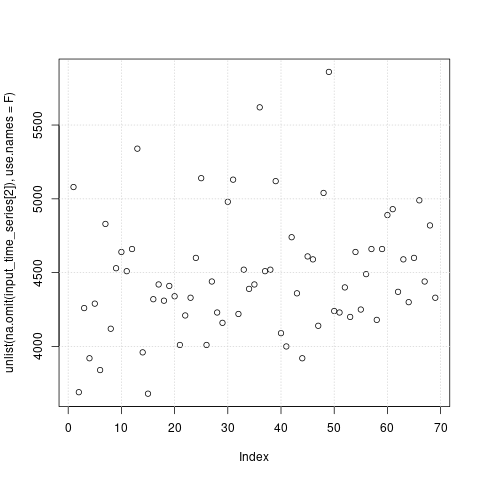
\includegraphics[width=.9\linewidth]{plot2.png}
        \caption{Dane zaszumione}
        \label{fig:sfig1}
    \end{subfigure}
    \begin{subfigure}{.5\textwidth}
        \centering
        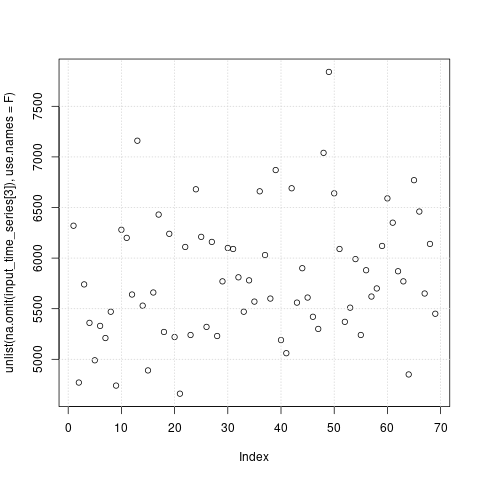
\includegraphics[width=.9\linewidth]{plot3.png}
        \caption{Dane zaszumione}
        \label{fig:sfig2}
    \end{subfigure}
    \begin{subfigure}{.5\textwidth}
        \centering
        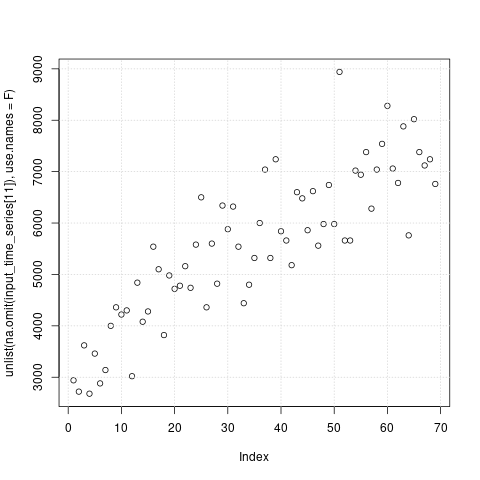
\includegraphics[width=.9\linewidth]{plot11.png}
        \caption{Trend}
        \label{fig:sfig3}
    \end{subfigure}
    \begin{subfigure}{.5\textwidth}
        \centering
        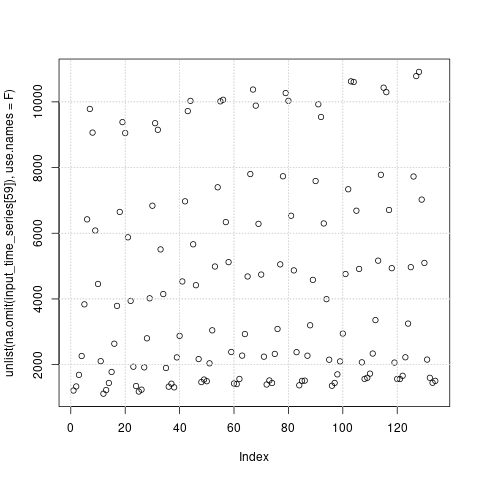
\includegraphics[width=.9\linewidth]{plot59.png}
        \caption{Wahania okresowe}
        \label{fig:sfig4}
    \end{subfigure}

    \caption{Przykładowe szeregi czasowe z benchmark'u NN3.}
    \label{fig:sample_time_series}
\end{figure}

Szeregi czasowe w benchmark'u NN3 są stosunkowo krótkie (min 68, max 144), a sam benchmark uznawany jest przez ekspertów z dzedziny modelowania szeregów czasowych jako dość ,,prosty''.

\section{Implementacja}

Szeregi czasowe z benchmark'u NN3 zostały znormalizowane do przedziału $<1:2>$ w celu umożliwienia porównywania błędów bezwzględnych.
Wadą normalizacji może być przeskalowanie większości z wartości szeregu do wąskiego przedziału w przypadku, kiedy w danych znajduje się co najmniej 1 mocno odstający punkt \cite{noauthor_standardization_nodate}.
Przesunięcie zakresu z przedziału $<0:1>$ do $<1:2>$ pozwala również na obliczanie błędów względnych bez obawy dzielenia przez 0.

Predykcja wartości odbywa się z krokiem o długości 1.
Oznacza to, iż przy predykcji wartości dla chwil czasowych $t+n$ wykorzystywane są rzeczywiste wartości szeregu z chwil czasowych wcześniejszych od $t+n$.

\subsection{ARIMA}
\textcolor{red}{Do uzupełnienia.}

\subsection{XGBoost}
\textcolor{red}{Do uzupełnienia.}

\section{Prezentacja wyników}
\color{red}
Porównanie modelu ARIMA z metodą xgboost dokonane zostanie na podstawie przebiegu funkcji gęstości prawdopodobieństwa względnych błędów.
Wartości błędów nie będą uśredniane dla poszczególnych szeregów, co oznacza, że długość wektora błędów dla którego zostanie przedstawiony przebieg funkcji gęstości prawdopodobieństwa wynosić będzie $111 \times 18 = 1998$.

Zagregowana funkcja gęstości prawdopodobieństwa błędów może ukrywać niektóre właściwości stosowanych modeli, dlatego zostanie ukazany również, na wspólnym  wykresie, przebieg błędów dla wszystkich szeregów czasowych.

Wyniki strojenia parametrów metody xgboost zaprezentowane zostaną w analogiczny sposób.
Dodatkowo zamieszczone mogą zostać fragmenty wydruków stosowanych funkcji, niosące wartościowe informacje.

\bibliographystyle{plain}
\bibliography{MEUM_projekt.bib}

\end{document}
